\chapter{LED Push Button Microcontroller}
\section{Introduction}
A \gls{led} push button microcontroller is a specialized electronic device designed to request the direction of a turnout be changed and to display the satus of the turnouts assigned to the panel. These devices are essential in model railroading and railway automation, where precise and reliable control of turnouts is required. By using a microcontroller, it is possible to automate the operation of turnouts, integrate them into larger control systems, and provide feedback on their status. This chapter discusses the design and implementation of a microcontroller-based system for the lights and push buttons of a turnout panel.
\begin{figure}[H]
  \centering
    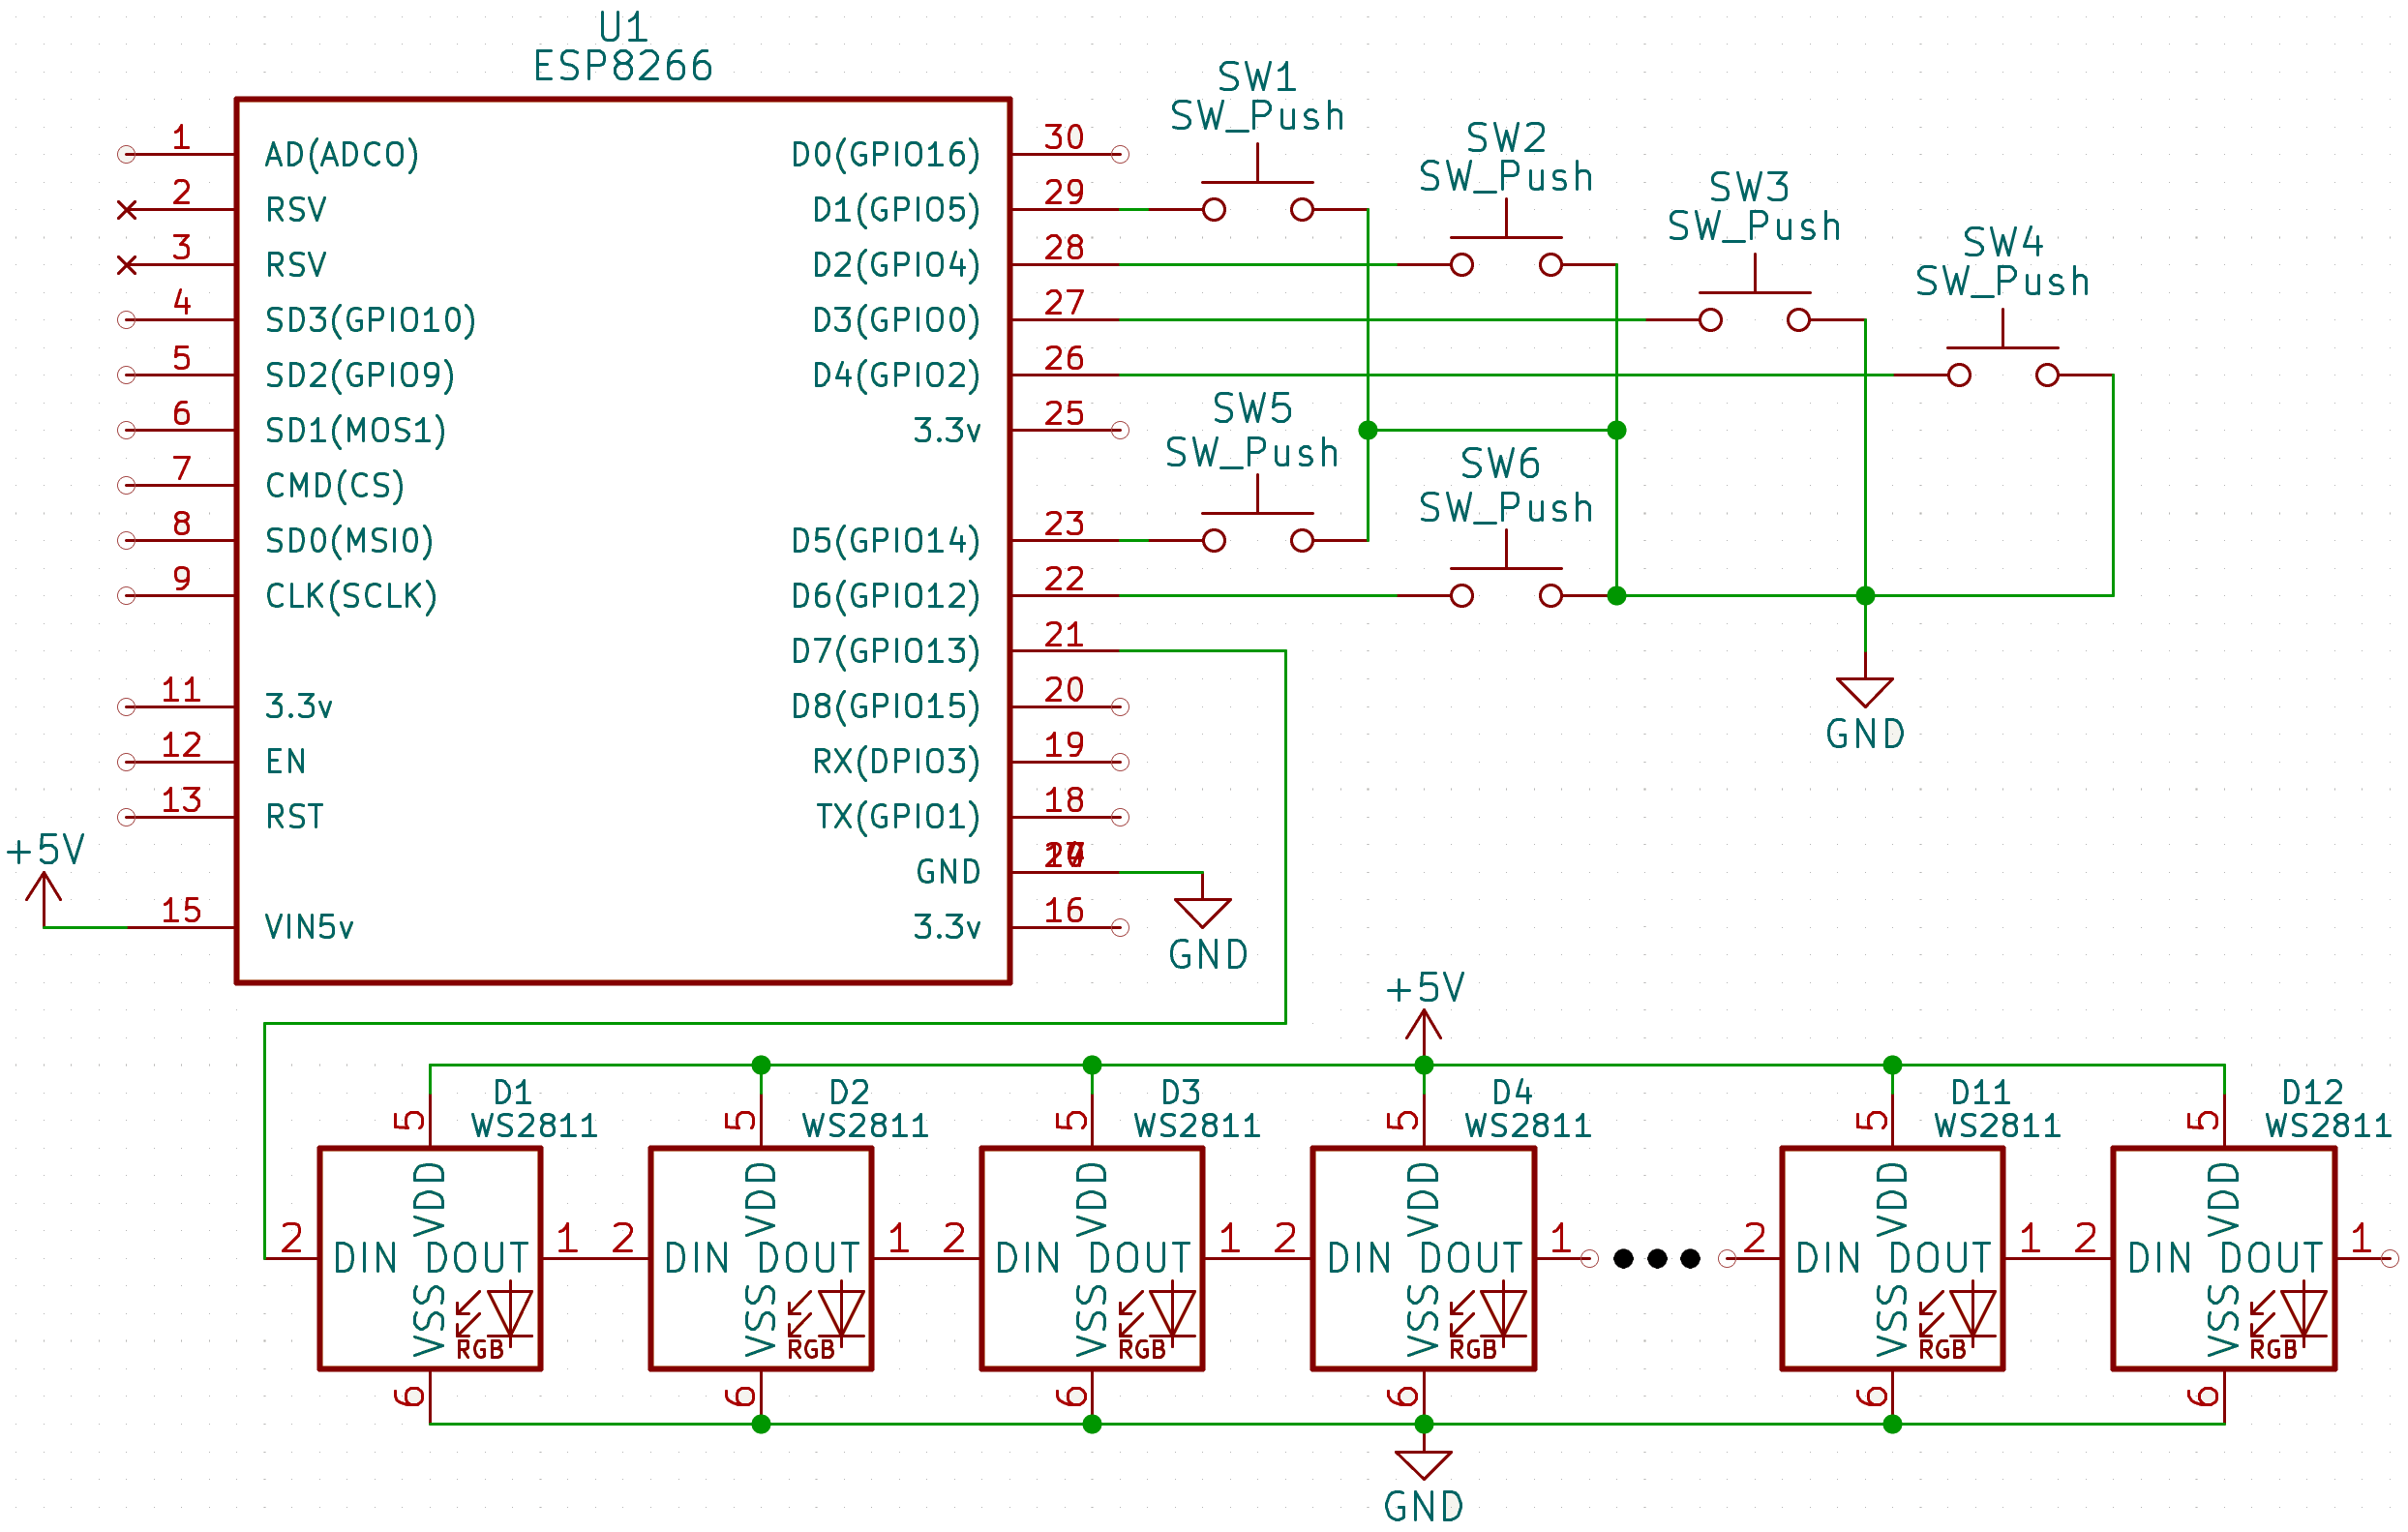
\includegraphics[scale=0.18]{../Images/lpb_schematic.png}
  \caption{LED Push Button Microcontroller Schematic}
  \label{fig:lpb-schematic}
\end{figure}

The hardware used in the \gls{led} push button microcontroller circuit consists of several components that work together to control a chain of 12 \glspl{led} and react to 6 push buttons. The main components are:
\begin{itemize}
\item NodeMCU (U1) is an ESP8266-based development board, which controls the other components.
\item Buttons (SW1 - SW6) There are six momentary push buttons. Each button connects a specific \gls{gpio} pin on the ESP8266 to \gls{gnd}. When a button is pressed, it creates a connection to ground, and the microcontroller detects this change. Each button press initiates a request to change the direction of the associated turnout.
\item LED Strip (D1 - D12) The circuit is designed to control a chain of 12 addressable \glspl{led}, of the WS2811 type. Each pair of \glspl{led} represents the status of an associated turnout.
\end{itemize}

The ESP8266 microcontroller reads the state of the buttons, which represents a specific turnout. The microcontroller controls the color of the \glspl{led}.
\section{Software}
The software for the \gls{led} push button microcontroller is developed using the \gls{vscode}, which provides a user-friendly environment for programming microcontrollers. The code is written in C/C++ and utilizes various libraries to facilitate communication with the components. The software implementation includes the following key functionalities:
\begin{itemize}
    \item Initialization of the NodeMCU and configuration of the GPIO pins.
    \item Initialization of the \gls{wifi} connectivity and connect to the \gls{mqtt} broker. This allows the microcontroller to send and receive messages over the network. At the finish of the initialization process, the microcontroller will publish a message to the topic ``micros''  indicating its readiness and status to the \gls{mqtt} broker. The message is in \gls{json} format as follows:\\
\{``et'':``1590462747'':``mcntrlr'':``LpbCntlr01'':``msgType'':``initial'':``ip'':``192.168.0.19''\}
    \item Subscribes to the topic acts/tpl/LpbCntlrxx where xx is a specific controller from the \gls{mqtt} broker. The message is in \gls{json} format as follows:\\
\{``cntrlr'':``LpbCntlrxx'':``lamp'':``1|2|3...6'':``color'':``RED|GREEN|BLUE|YELLOW''\}
    \item Reads up to 6 buttons (count set in ``params.h'') using simple debouncing and publishes a \gls{json} message on press to the topic ``sensors/pb'' to the \gls{mqtt} broker. The message is in \gls{json} format as follows:\\
    \{``et'':``1590462747'':``mcntrlr'':``LpbCntlrxx'':``pb'':``1|2|3...6''\}
    \item Locks that button until a command arrives on the command topic with a matching ``lamp'' number is recieved.
    \item Sending periodic heartbeat messages to the \gls{mqtt} broker to indicate that the microcontroller is operational. This can be used for monitoring and debugging purposes. The message are in \gls{json} format as follows:\\
\{``et'':``1590462747'',``mcntrlr'':``LpbCntlrxx'',``msgType'':``heartbeat''\}
\end{itemize}
The software is designed to be modular and easily maintainable, allowing for future enhancements and bug fixes. The use of libraries such as ``Adafruit\_NeoPixel.h'' for control of WS2811 \gls{led} strip and ``PubSubClient.h'' for \gls{mqtt} messaging simplifies the implementation and ensures compatibility with the hardware components.

